
\subsection{Διαγράμματα και πίνακες παραμέτρων για κάθε μηχανικό μοντέλο}

\subsubsection{Όλα τα δεδομένα}

\begin{figure}[!htbp]
    \centering

    % --- Three smaller images ---
    \begin{minipage}{0.3\textwidth}
        \centering
        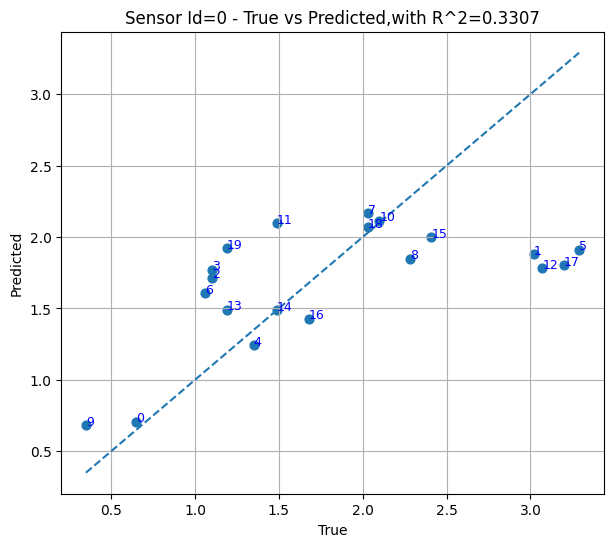
\includegraphics[width=\textwidth]{εικόνες/αποτελέσματα μηχανικών μοντέλων/All data/0_plots.png}
    \end{minipage}
    \hfill
    \begin{minipage}{0.3\textwidth}
        \centering
        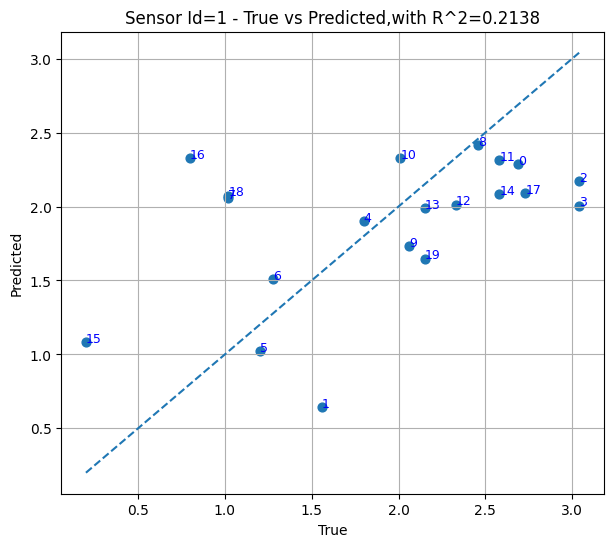
\includegraphics[width=\textwidth]{εικόνες/αποτελέσματα μηχανικών μοντέλων/All data/1_plots.png}
    \end{minipage}
    \hfill
    \begin{minipage}{0.3\textwidth}
        \centering
        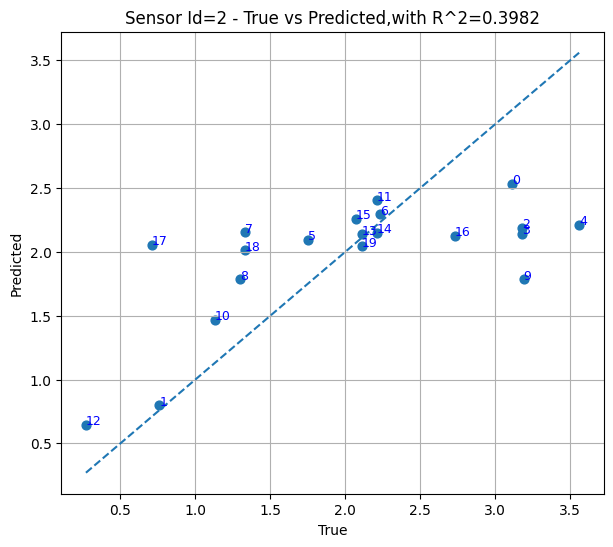
\includegraphics[width=\textwidth]{εικόνες/αποτελέσματα μηχανικών μοντέλων/All data/2_plots.png}
    \end{minipage}

    \vspace{0.5cm}

    % --- Large prominent image ---
    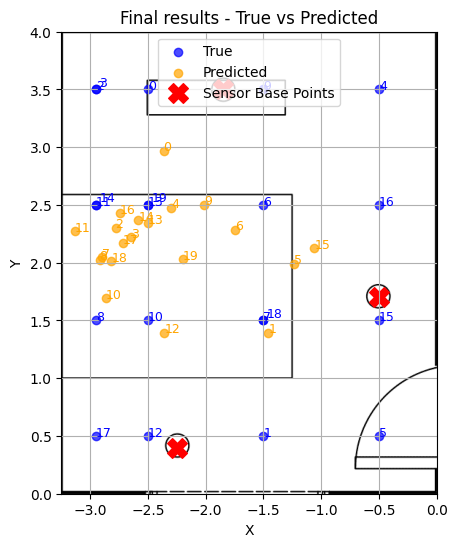
\includegraphics[  width=0.70\textwidth,
        height=0.40\textheight,
        keepaspectratio]{εικόνες/αποτελέσματα μηχανικών μοντέλων/All data/Final_plots.png}

    \caption{Όχι Διαχείριση Outliers}
    \label{fig:all_data_}

\end{figure}

\begin{figure}[!htbp]
    \centering

    % --- Three smaller images ---
    \begin{minipage}{0.3\textwidth}
        \centering
        
\includegraphics[width=\textwidth]{εικόνες/αποτελέσματα μηχανικών μοντέλων/All datacutOutliers/0_plots.png}
    \end{minipage}
    \hfill
    \begin{minipage}{0.3\textwidth}
        \centering
        
\includegraphics[width=\textwidth]{εικόνες/αποτελέσματα μηχανικών μοντέλων/All datacutOutliers/1_plots.png}
    \end{minipage}
    \hfill
    \begin{minipage}{0.3\textwidth}
        \centering
        
\includegraphics[width=\textwidth]{εικόνες/αποτελέσματα μηχανικών μοντέλων/All datacutOutliers/2_plots.png}
    \end{minipage}

    \vspace{0.5cm}

    % --- Large prominent image ---
    
\includegraphics[  width=0.70\textwidth,
        height=0.40\textheight,
        keepaspectratio]{εικόνες/αποτελέσματα μηχανικών μοντέλων/All datacutOutliers/Final_plots.png}

    \caption{Διαχείριση Outliers σε συνολικό επίπεδο}
    \label{fig:all_data_Global_Outliers}

\end{figure}

\begin{figure}[!htbp]
    \centering

    % --- Three smaller images ---
    \begin{minipage}{0.3\textwidth}
        \centering
        
\includegraphics[width=\textwidth]{εικόνες/αποτελέσματα μηχανικών μοντέλων/All datacutOutliersPerColumn/0_plots.png}
    \end{minipage}
    \hfill
    \begin{minipage}{0.3\textwidth}
        \centering
        
\includegraphics[width=\textwidth]{εικόνες/αποτελέσματα μηχανικών μοντέλων/All datacutOutliersPerColumn/1_plots.png}
    \end{minipage}
    \hfill
    \begin{minipage}{0.3\textwidth}
        \centering
        
\includegraphics[width=\textwidth]{εικόνες/αποτελέσματα μηχανικών μοντέλων/All datacutOutliersPerColumn/2_plots.png}
    \end{minipage}

    \vspace{0.5cm}

    % --- Large prominent image ---
    
\includegraphics[  width=0.70\textwidth,
        height=0.40\textheight,
        keepaspectratio]{εικόνες/αποτελέσματα μηχανικών μοντέλων/All datacutOutliersPerColumn/Final_plots.png}

    \caption{Διαχείριση Outliers ανά στήλη}
    \label{fig:all_data_Outliers_Per_Column}

\end{figure}

\FloatBarrier
%--------------------------------------------------------------

\subsubsection{Πιο κοντινή πηγή ανά αισθητήρα}

\begin{figure}[!htbp]
    \centering

    % --- Three smaller images ---
    \begin{minipage}{0.3\textwidth}
        \centering
        
\includegraphics[width=\textwidth]{εικόνες/αποτελέσματα μηχανικών μοντέλων/close sources/0_plots.png}
    \end{minipage}
    \hfill
    \begin{minipage}{0.3\textwidth}
        \centering
        
\includegraphics[width=\textwidth]{εικόνες/αποτελέσματα μηχανικών μοντέλων/Close sources/1_plots.png}
    \end{minipage}
    \hfill
    \begin{minipage}{0.3\textwidth}
        \centering
        
\includegraphics[width=\textwidth]{εικόνες/αποτελέσματα μηχανικών μοντέλων/Close sources/2_plots.png}
    \end{minipage}

    \vspace{0.5cm}

    % --- Large prominent image ---
    
\includegraphics[  width=0.70\textwidth,
        height=0.40\textheight,
        keepaspectratio]{εικόνες/αποτελέσματα μηχανικών μοντέλων/Close sources/Final_plots.png}

    \caption{Όχι Διαχείριση Outliers}
    \label{fig:closest}

\end{figure}

\begin{figure}[!htbp]
    \centering

    % --- Three smaller images ---
    \begin{minipage}{0.3\textwidth}
        \centering
        
\includegraphics[width=\textwidth]{εικόνες/αποτελέσματα μηχανικών μοντέλων/Close sourcescutOutliers/0_plots.png}
    \end{minipage}
    \hfill
    \begin{minipage}{0.3\textwidth}
        \centering
        
\includegraphics[width=\textwidth]{εικόνες/αποτελέσματα μηχανικών μοντέλων/Close sourcescutOutliers/1_plots.png}
    \end{minipage}
    \hfill
    \begin{minipage}{0.3\textwidth}
        \centering
        
\includegraphics[width=\textwidth]{εικόνες/αποτελέσματα μηχανικών μοντέλων/Close sourcescutOutliers/2_plots.png}
    \end{minipage}

    \vspace{0.5cm}

    % --- Large prominent image ---
    
\includegraphics[  width=0.70\textwidth,
        height=0.40\textheight,
        keepaspectratio]{εικόνες/αποτελέσματα μηχανικών μοντέλων/Close sourcescutOutliers/Final_plots.png}

    \caption{Διαχείριση Outliers σε συνολικό επίπεδο}
    \label{fig:closest_Global_Outliers}

\end{figure}

\begin{figure}[!htbp]
    \centering

    % --- Three smaller images ---
    \begin{minipage}{0.3\textwidth}
        \centering
        
\includegraphics[width=\textwidth]{εικόνες/αποτελέσματα μηχανικών μοντέλων/Close sourcescutOutliersPerColumn/0_plots.png}
    \end{minipage}
    \hfill
    \begin{minipage}{0.3\textwidth}
        \centering
        
\includegraphics[width=\textwidth]{εικόνες/αποτελέσματα μηχανικών μοντέλων/Close sourcescutOutliersPerColumn/1_plots.png}
    \end{minipage}
    \hfill
    \begin{minipage}{0.3\textwidth}
        \centering
        
\includegraphics[width=\textwidth]{εικόνες/αποτελέσματα μηχανικών μοντέλων/Close sourcescutOutliersPerColumn/2_plots.png}
    \end{minipage}

    \vspace{0.5cm}

    % --- Large prominent image ---
    
\includegraphics[  width=0.70\textwidth,
        height=0.40\textheight,
        keepaspectratio]{εικόνες/αποτελέσματα μηχανικών μοντέλων/Close sourcescutOutliersPerColumn/Final_plots.png}

    \caption{Διαχείριση Outliers ανά στήλη}
    \label{fig:closest_Outliers_Per_Column}

\end{figure}
\FloatBarrier

%--------------------------------------------------------------

\subsubsection{Δύο πιο κοντινές πηγές ανά αισθητήρα}

\begin{figure}[!htbp]
    \centering

    % --- Three smaller images ---
    \begin{minipage}{0.3\textwidth}
        \centering
        
\includegraphics[width=\textwidth]{εικόνες/αποτελέσματα μηχανικών μοντέλων/second close sources/0_plots.png}
    \end{minipage}
    \hfill
    \begin{minipage}{0.3\textwidth}
        \centering
        
\includegraphics[width=\textwidth]{εικόνες/αποτελέσματα μηχανικών μοντέλων/second close sources/1_plots.png}
    \end{minipage}
    \hfill
    \begin{minipage}{0.3\textwidth}
        \centering
        
\includegraphics[width=\textwidth]{εικόνες/αποτελέσματα μηχανικών μοντέλων/second close sources/2_plots.png}
    \end{minipage}

    \vspace{0.5cm}

    % --- Large prominent image ---
    
\includegraphics[  width=0.70\textwidth,
        height=0.40\textheight,
        keepaspectratio]{εικόνες/αποτελέσματα μηχανικών μοντέλων/second close sources/Final_plots.png}

    \caption{Όχι Διαχείριση Outliers}
    \label{fig:two_closest}

\end{figure}

\begin{figure}[!htbp]
    \centering

    % --- Three smaller images ---
    \begin{minipage}{0.3\textwidth}
        \centering
        
\includegraphics[width=\textwidth]{εικόνες/αποτελέσματα μηχανικών μοντέλων/second close sourcescutOutliers/0_plots.png}
    \end{minipage}
    \hfill
    \begin{minipage}{0.3\textwidth}
        \centering
        
\includegraphics[width=\textwidth]{εικόνες/αποτελέσματα μηχανικών μοντέλων/second close sourcescutOutliers/1_plots.png}
    \end{minipage}
    \hfill
    \begin{minipage}{0.3\textwidth}
        \centering
        
\includegraphics[width=\textwidth]{εικόνες/αποτελέσματα μηχανικών μοντέλων/second close sourcescutOutliers/2_plots.png}
    \end{minipage}

    \vspace{0.5cm}

    % --- Large prominent image ---
    
\includegraphics[  width=0.70\textwidth,
        height=0.40\textheight,
        keepaspectratio]{εικόνες/αποτελέσματα μηχανικών μοντέλων/second close sourcescutOutliers/Final_plots.png}

    \caption{Διαχείριση Outliers σε συνολικό επίπεδο}
    \label{fig:two_closest_Global_Outliers}

\end{figure}

\begin{figure}[!htbp]
    \centering

    % --- Three smaller images ---
    \begin{minipage}{0.3\textwidth}
        \centering
        
\includegraphics[width=\textwidth]{εικόνες/αποτελέσματα μηχανικών μοντέλων/second close sourcescutOutliersPerColumn/0_plots.png}
    \end{minipage}
    \hfill
    \begin{minipage}{0.3\textwidth}
        \centering
        
\includegraphics[width=\textwidth]{εικόνες/αποτελέσματα μηχανικών μοντέλων/second close sourcescutOutliersPerColumn/1_plots.png}
    \end{minipage}
    \hfill
    \begin{minipage}{0.3\textwidth}
        \centering
        
\includegraphics[width=\textwidth]{εικόνες/αποτελέσματα μηχανικών μοντέλων/second close sourcescutOutliersPerColumn/2_plots.png}
    \end{minipage}

    \vspace{0.5cm}

    % --- Large prominent image ---
    
\includegraphics[  width=0.70\textwidth,
        height=0.40\textheight,
        keepaspectratio]{εικόνες/αποτελέσματα μηχανικών μοντέλων/second close sourcescutOutliersPerColumn/Final_plots.png}

    \caption{Διαχείριση Outliers ανά στήλη}
    \label{fig:two_closest_Outliers_Per_Column}

\end{figure}

\FloatBarrier
